%%
%% Copyright 2007, 2008, 2009 Elsevier Ltd
%%
%% This file is part of the 'Elsarticle Bundle'.
%% ---------------------------------------------
%%
%% It may be distributed under the conditions of the LaTeX Project Public
%% License, either version 1.2 of this license or (at your option) any
%% later version.  The latest version of this license is in
%%    http://www.latex-project.org/lppl.txt
%% and version 1.2 or later is part of all distributions of LaTeX
%% version 1999/12/01 or later.
%%
%% The list of all files belonging to the 'Elsarticle Bundle' is
%% given in the file `manifest.txt'.
%%

%% Template article for Elsevier's document class `elsarticle'
%% with numbered style bibliographic references
%% SP 2008/03/01
%%
%%
%%
%% $Id: elsarticle-template-num.tex 4 2009-10-24 08:22:58Z rishi $
%%
%%
%\documentclass[preprint,12pt]{elsarticle}

%% Use the option review to obtain double line spacing
%\documentclass[preprint,review,12pt]{elsarticle}
\documentclass[preprint,10pt]{elsarticle}

%% Use the options 1p,twocolumn; 3p; 3p,twocolumn; 5p; or 5p,twocolumn
%% for a journal layout:
%% \documentclass[final,1p,times]{elsarticle}
%% \documentclass[final,1p,times,twocolumn]{elsarticle}
%% \documentclass[final,3p,times]{elsarticle}
%% \documentclass[final,3p,times,twocolumn]{elsarticle}
%% \documentclass[final,5p,times]{elsarticle}
%% \documentclass[final,5p,times,twocolumn]{elsarticle}

%% if you use PostScript figures in your article
%% use the graphics package for simple commands
%% \usepackage{graphics}
%% or use the graphicx package for more complicated commands
%% \usepackage{graphicx}
%% or use the epsfig package if you prefer to use the old commands
%% \usepackage{epsfig}
%%%%%%%%%%%%%%%%%%%%%%%%%%%%%%%%%%%%%%%%%%%%%%%%%%%%%%%%%%%%%%%%%%%%
%% Package Listing
\usepackage{color}
\usepackage{graphicx}
\usepackage{amssymb}
\usepackage{amsmath}
\usepackage{amsfonts}
\usepackage{amstext}
\usepackage{amsbsy}
\usepackage{subcaption}
\usepackage{epstopdf}
%%%%%%%%%%%%%%%%%%%%%%%%%%%%%%%%%%%%%%%%%%%%%%%%%%%%%%%%%%%%%%%%%%%%
%% The lineno packages adds line numbers. Start line numbering with
%% \begin{linenumbers}, end it with \end{linenumbers}. Or switch it on
%% for the whole article with \linenumbers after \end{frontmatter}.
\usepackage{lineno}
%%%%%%%%%%%%%%%%%%%%%%%%%%%%%%%%%%%%%%%%%%%%%%%%%%%%%%%%%%%%%%%%%%%%
% DGFEM commands
\newcommand{\jmp}[1]{[\![#1]\!]}                     % jump
\newcommand{\mvl}[1]{\{\!\!\{#1\}\!\!\}}             % mean value
\newcommand{\keff}{\ensuremath{k_{\textit{eff}}}\xspace}
%% Other Commands
\newcommand{\tcr}[1]{\textcolor{red}{#1}}
\newcommand{\mt}[1]{\marginpar{ {\tiny #1}}}
\newcommand{\Introfigpath}[1]{../../../Document/Rev0/figures/sec_Intro/{#1}}
\newcommand{\Snfigpath}[1]{../../../Document/Rev0/figures/sec_Sn/{#1}}
\newcommand{\BFfigpath}[1]{../../../Document/Rev0/figures/sec_BF/{#1}}
\newcommand{\DSAfigpath}[1]{../../../Document/Rev0/figures/sec_DSA/{#1}}
%%%%%%%%%%%%%%%%%%%%%%%%%%%%%%%%%%%%%%%%%%%%%%%%%%%%%%%%%%%%%%%%%%%%
\journal{Nuclear Science and Engineering}

\begin{document}
%-------------------------
\begin{frontmatter}
%-------------------------
\title{Parellelizable Methodology for Accelerating Thermal Neutron Upscattering}
%-------------------------
\author{Michael W. Hackemack}
\author{Jean C. Ragusa}
\ead{jean.ragusa@tamu.edu}
\address{Department of Nuclear Engineering, Texas A\&M University, College Station, TX 77843, USA}
%-------------------------
\begin{abstract}
%% Text of abstract
abstract goes here...
\end{abstract}
%-------------------------
\begin{keyword}
Thermal Neutron Upscattering \sep Two-Grid \sep DSA \sep Parallel \sep Jacobi
\end{keyword}
%-------------------------
\end{frontmatter}
%-------------------------
%%%%%%%%%%%%%%%%%%%%%%%%%%%%%%%%%%%%%%%%%%%%%%%%%%%%%%%%%%%%%%%%%%%%

\linenumbers

%%%%%%%%%%%%%%%%%%%%%%%%%%%%%%%%%%%%%%%%%%%%%%%%%%%%%%%%%%%%%%%%%%%%
%%%%%%%%%%%%%%%%%%%%%%%%%%%%%%%%%%%%%%%%%%%%%%%%%%%%%%%%%%%%%%%%%%%%
\section{Introduction} \label{sec::intro}
%%%%%%%%%%%%%%%%%%%%%%%%%%%%%%%%%%%%%%%%%%%%%%%%%%%%%%%%%%%%%%%%%%%%
%%%%%%%%%%%%%%%%%%%%%%%%%%%%%%%%%%%%%%%%%%%%%%%%%%%%%%%%%%%%%%%%%%%%

\tcr
{
\begin{enumerate}
\item Brief description of outer-iteration scheme for multigroup problems (words only). Historically (and still used today in several software, ref, simulate ), this was a GS procedure (note: some recent works build athe full MG unsymmetric matrix, rattlesnake, parcs). Why is acceleration of GS important? D2O, C.
transition to previous work on acceleration of GS
\item Historical upscatter acceleration work:
\begin{itemize}
\item: start with TG 1993, in passing Averin+Vol., MTG, MF-grey (was this before TG?). As closing, other techniques used iteration residuals (including thermal upscatter residual), e.g., Sanchez et al. (point out not converging innners outers in the fission accel)
\item multifrequency-grey
\item Fission source acceleration
\item Averin and Voloschenko upscatter (nonlinear procedure)
\item Finally, TG and MTG. Can mention that Evans and Clarno specifically came up with TTG because MIP had not been developed and it wasn't known if a DSA scheme would be stable for unstructured multi-dimensional and multi-material problems.
\end{itemize}
\item Describe desire for parallelizable acceleration methodology motivated by massively-parallel computer architectures. Sn transport sweeps. Shameless plug for PDT (with references)  Mention that our methods were motivated by the TG and MTG methods.
\item outline (sell your ANALYSIS work too, not just the numerical PDT results)
\end{enumerate}
}

%%%%%%%%%%%%%%%%%%%%%%%%%%%%%%%%%%%%%%%%%%%%%%%%%%%%%%%%%%%%%%%%%%%%
%%%%%%%%%%%%%%%%%%%%%%%%%%%%%%%%%%%%%%%%%%%%%%%%%%%%%%%%%%%%%%%%%%%%
\section{Serial Gauss-Seidel Acceleration Methodologies} \label{sec::GS}
%%%%%%%%%%%%%%%%%%%%%%%%%%%%%%%%%%%%%%%%%%%%%%%%%%%%%%%%%%%%%%%%%%%%
%%%%%%%%%%%%%%%%%%%%%%%%%%%%%%%%%%%%%%%%%%%%%%%%%%%%%%%%%%%%%%%%%%%%

%------------------------------------------------------------------------------------------------------------
\subsection{Two-Grid Acceleration}
%------------------------------------------------------------------------------------------------------------

\tcr{Give the outline of the TG method. This section would be a little longer since it would need to introduce the factorized error mode, the averaged diffusion equation, and the group-dependent update.}

give once TE fully spelled out (no ang/space disct) but multigroup. quickly introduce operator notations. make a note about Sn in angle DFEM in space (ref).

talk about that one eigenvalue close to 1 of the iteration process that the 2grid acceleration was killing.

%------------------------------------------------------------------------------------------------------------
\subsection{Modified Two-Grid Acceleration}
%------------------------------------------------------------------------------------------------------------
MTG: Evans used transport for the energy-collapsed equation. here, we present it for one-group diffusion since this is how we apply it. because now we have reliable diffusion accelerator...
\tcr
{
state differences with TG (this should be relatively short):
\begin{enumerate}
\item 1 sweep per group in GS procedure
\item spectral shape collapse eigenvalue equation
\item low-order residual
\end{enumerate}
}
message: silly to converge inners before going to next thermal group. however, account for non-convergence of inners through spectrally collapsed residual in the 1-g acceleration.

%%%%%%%%%%%%%%%%%%%%%%%%%%%%%%%%%%%%%%%%%%%%%%%%%%%%%%%%%%%%%%%%%%%%
%%%%%%%%%%%%%%%%%%%%%%%%%%%%%%%%%%%%%%%%%%%%%%%%%%%%%%%%%%%%%%%%%%%%
\section{Parallelizable Jacobi Acceleration Methodologies} \label{sec::Jac}
%%%%%%%%%%%%%%%%%%%%%%%%%%%%%%%%%%%%%%%%%%%%%%%%%%%%%%%%%%%%%%%%%%%%
%%%%%%%%%%%%%%%%%%%%%%%%%%%%%%%%%%%%%%%%%%%%%%%%%%%%%%%%%%%%%%%%%%%%

\tcr{Discuss desire to simultaneously solve transport sweeps. Propose the two Jacobi methods in the same mold as the GS methods (Modified means to not converge the inners).}

\tcr
{
per our discussion of the story flow:
1. MTG-GS: not good for // \\
2. thus go with MTG-Jacobi. not converging the inners (inspired by MTG-GS) but accounting for them in the spectrally-averaged residual \\. 
3. gains in // can be expected (to be verified with FA + num results). however, is spectral collapse acceleration (2-grid) doing a good job? can we boost it? because converging the inners with TG-GS was excellent. however, we do not want to sweep. idea. good enough convergence in the form of a DSA per group.
}

%------------------------------------------------------------------------------------------------------------
\subsection{Jacobi Acceleration}
%------------------------------------------------------------------------------------------------------------
\tcr
{
\begin{enumerate}
\item we do not want to converge inners with sweeps (would be silly to not communicate after each iteration)
\item want to estimate convergence of inners with a within-group DSA acceleration for each group
\item finish with spectrally-collapsed acceleration step
\end{enumerate}
}

%------------------------------------------------------------------------------------------------------------
\subsection{Modified Jacobi Acceleration}
%------------------------------------------------------------------------------------------------------------

\tcr{describe small difference with the Jacobi Acceleration which is the removal of the middle step (the within-group accelerations)}

%%%%%%%%%%%%%%%%%%%%%%%%%%%%%%%%%%%%%%%%%%%%%%%%%%%%%%%%%%%%%%%%%%%%
%%%%%%%%%%%%%%%%%%%%%%%%%%%%%%%%%%%%%%%%%%%%%%%%%%%%%%%%%%%%%%%%%%%%
\section{Summary of Upscatter Acceleration Methodologies} \label{sec::summary}
%%%%%%%%%%%%%%%%%%%%%%%%%%%%%%%%%%%%%%%%%%%%%%%%%%%%%%%%%%%%%%%%%%%%
%%%%%%%%%%%%%%%%%%%%%%%%%%%%%%%%%%%%%%%%%%%%%%%%%%%%%%%%%%%%%%%%%%%%

\tcr{summarize/uniform naming and put a table with acronyms}

%%%%%%%%%%%%%%%%%%%%%%%%%%%%%%%%%%%%%%%%%%%%%%%%%%%%%%%%%%%%%%%%%%%%
%%%%%%%%%%%%%%%%%%%%%%%%%%%%%%%%%%%%%%%%%%%%%%%%%%%%%%%%%%%%%%%%%%%%
\section{The Modified Interior Penalty Method} \label{sec::MIP}
%%%%%%%%%%%%%%%%%%%%%%%%%%%%%%%%%%%%%%%%%%%%%%%%%%%%%%%%%%%%%%%%%%%%
%%%%%%%%%%%%%%%%%%%%%%%%%%%%%%%%%%%%%%%%%%%%%%%%%%%%%%%%%%%%%%%%%%%%

\tcr{BRIEF overview of the MIP discretization with appropriate references. Turcksin and Ragusa is a short and straightforward presentation of MIP to base on.}

TEXT TEXT TEXT. IP DFEM, used as DSA, works well (cite) (at most, bilinear form for MIP in appendix).
% MIP-DSA works in //: PhD dissertation as ref, if needed until other paper is done

%%%%%%%%%%%%%%%%%%%%%%%%%%%%%%%%%%%%%%%%%%%%%%%%%%%%%%%%%%%%%%%%%%%%
%%%%%%%%%%%%%%%%%%%%%%%%%%%%%%%%%%%%%%%%%%%%%%%%%%%%%%%%%%%%%%%%%%%%
\section{Numerical Results} \label{sec::results}
%%%%%%%%%%%%%%%%%%%%%%%%%%%%%%%%%%%%%%%%%%%%%%%%%%%%%%%%%%%%%%%%%%%%
%%%%%%%%%%%%%%%%%%%%%%%%%%%%%%%%%%%%%%%%%%%%%%%%%%%%%%%%%%%%%%%%%%%%
\tcr{sell out stuff: you ground your work in ANALYSIS not trial and error. (note: say it in the intro too!). Shameless plug for PDT.}

%------------------------------------------------------------------------------------------------------------
\subsection{Theoretical Analysis}
%------------------------------------------------------------------------------------------------------------
\tcr{Fourier and flat mode plots for the different methods.}


4 spectral shapes for graphite plot

% Graphite spectral shapes
% ------------------------------
\begin{figure}
\centering
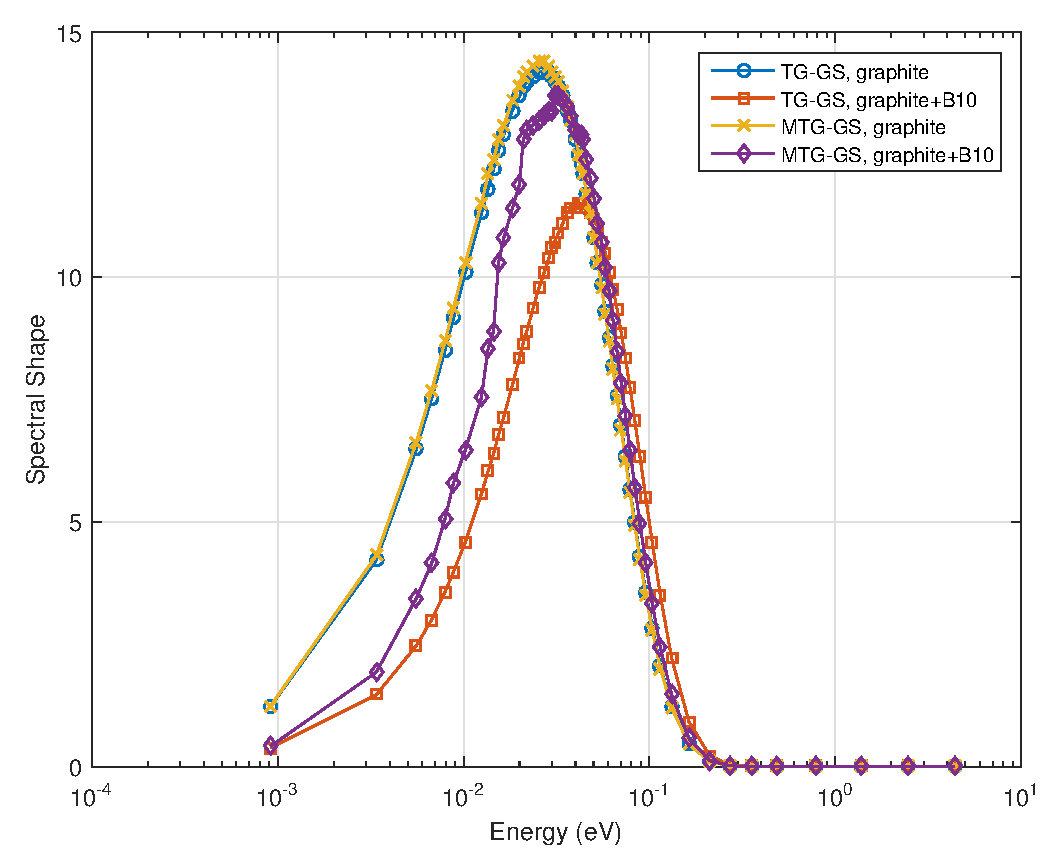
\includegraphics[width=0.85\textwidth]{figures/SS_GS_graphite.eps}
\caption{Spectral shapes of the Gauss-Seidel methods for pure graphite and graphite with 50 ppm of boron.}
\label{fig::Flat_FA_TGandMTG}
\end{figure}

\begin{figure}
\centering
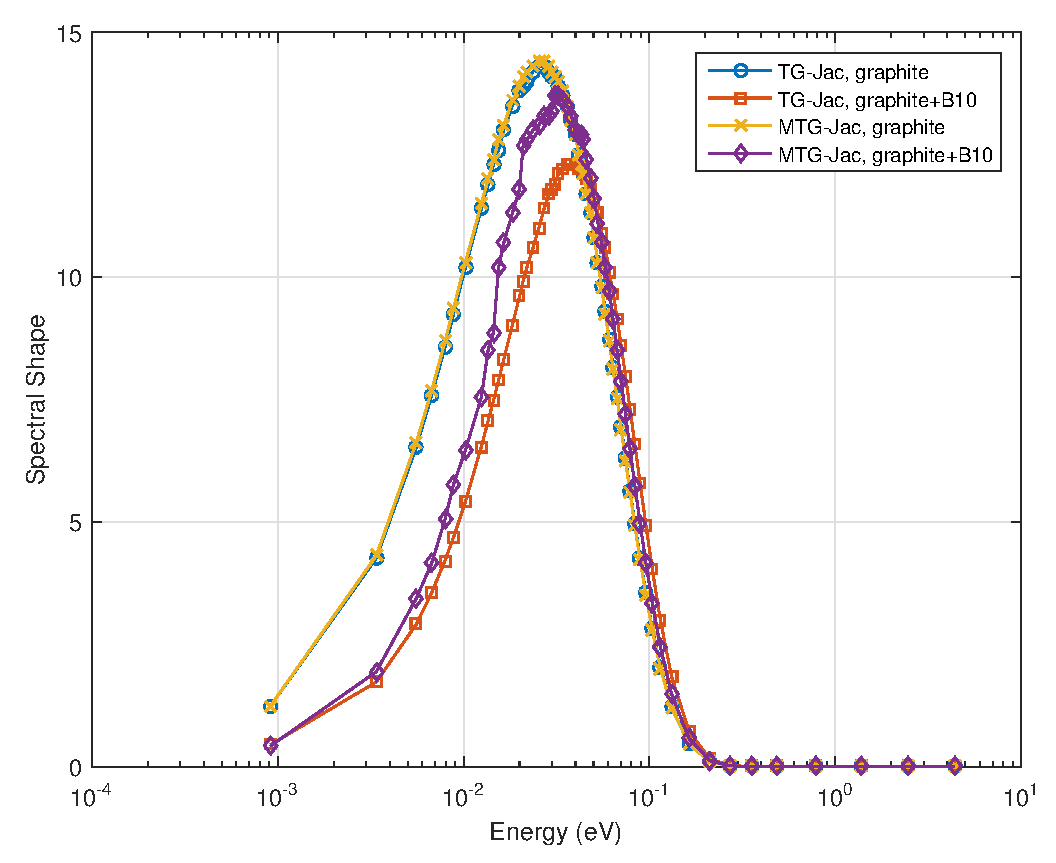
\includegraphics[width=0.85\textwidth]{figures/SS_Jac_graphite.eps}
\caption{Spectral shapes of the Jacobi methods for pure graphite and graphite with 50 ppm of boron.}
\label{fig::Flat_FA_TGandMTG}
\end{figure}
% ------------------------------

% Flat-mode eigenvalues
% ---------------------------
\begin{figure}
\centering
	\begin{subfigure}[b]{0.80\textwidth}
		\centering
		\includegraphics[width=0.975\textwidth]{\DSAfigpath{IM1_Graph_FA_TG.eps}}
		\caption{Two-Grid}
	\end{subfigure}
	
	\begin{subfigure}[b]{0.80\textwidth}
		\centering
		\includegraphics[width=0.975\textwidth]{\DSAfigpath{IM1_Graph_FA_MTG.eps}}
		\caption{Modified Two-Grid}
	\end{subfigure}
\caption{Flat mode eigenvalues for the TG-GS and MTG-GS schemes.}
\label{fig::Flat_FA_TGandMTG}
\end{figure}

\begin{figure}
\centering
	\begin{subfigure}[b]{0.80\textwidth}
		\centering
		\includegraphics[width=0.975\textwidth]{\DSAfigpath{IM1_Graph_FA_MJA.eps}}
		\caption{Modified Jacobi Acceleration}
	\end{subfigure}
	
	\begin{subfigure}[b]{0.80\textwidth}
		\centering
		\includegraphics[width=0.975\textwidth]{\DSAfigpath{IM1_Graph_FA_MJIA.eps}}
		\caption{Jacobi Acceleration}
	\end{subfigure}
\caption{Flat mode eigenvalues for the TG-Jac and MTG-Jac schemes.}
\label{fig::Flat_FA_MJAandMJIA}
\end{figure}
% ---------------------------

%------------------------------------------------------------------------------------------------------------
\subsection{Homogeneous Graphite Configuration}
%------------------------------------------------------------------------------------------------------------
\tcr{I was thinking a simple table with iteration statistics for a homogenous cube problem.}

\tcr{expectations: these results will match closely the FA results.}

%------------------------------------------------------------------------------------------------------------
\subsection{Heterogeneous Configurations}
%------------------------------------------------------------------------------------------------------------

\tcr{2D and 3D IM1 results}

\tcr{make a note on the highly heterogeneous configuration for which it is well known that ``all'' diffusion based accelerator have trouble, see Warsa/Yaqi ``PHI''.}
 

%%%%%%%%%%%%%%%%%%%%%%%%%%%%%%%%%%%%%%%%%%%%%%%%%%%%%%%%%%%%%%%%%%%%
%%%%%%%%%%%%%%%%%%%%%%%%%%%%%%%%%%%%%%%%%%%%%%%%%%%%%%%%%%%%%%%%%%%%
\section{Conclusions} \label{sec::conclusions}
%%%%%%%%%%%%%%%%%%%%%%%%%%%%%%%%%%%%%%%%%%%%%%%%%%%%%%%%%%%%%%%%%%%%
%%%%%%%%%%%%%%%%%%%%%%%%%%%%%%%%%%%%%%%%%%%%%%%%%%%%%%%%%%%%%%%%%%%%

In this paper,

%%%%%%%%%%%%%%%%%%%%%%%%%%%%%%%%%%%%%%%%%%%%%%%%%%%%%%%%%%%%%%%%%%%%
%%%%%%%%%%%%%%%%%%%%%%%%%%%%%%%%%%%%%%%%%%%%%%%%%%%%%%%%%%%%%%%%%%%%
\section*{Acknowledgments} 
%%%%%%%%%%%%%%%%%%%%%%%%%%%%%%%%%%%%%%%%%%%%%%%%%%%%%%%%%%%%%%%%%%%%
%%%%%%%%%%%%%%%%%%%%%%%%%%%%%%%%%%%%%%%%%%%%%%%%%%%%%%%%%%%%%%%%%%%%
This research was performed under appointment to the Rickover Graduate Fellowship Program in Nuclear Engineering sponsored by the Naval Reactors Division of the United States Department of Energy.

%%%%%%%%%%%%%%%%%%%%%%%%%%%%%%%%%%%%%%%%%%%%%%%%%%%%%%%%%%%%%%%%%%%%
%%%%%%%%%%%%%%%%%%%%%%%%%%%%%%%%%%%%%%%%%%%%%%%%%%%%%%%%%%%%%%%%%%%%
%%%%%%%%%%%%%%%%%%%%%%%%%%%%%%%%%%%%%%%%%%%%%%%%%%%%%%%%%%%%%%%%%%%%
%%%%%%%%%%%%%%%%%%%%%%%%%%%%%%%%%%%%%%%%%%%%%%%%%%%%%%%%%%%%%%%%%%%%
\bibliographystyle{elsarticle-num}
\bibliography{references}

% Begin appendices
\appendix
%%%%%%%%%%%%%%%%%%%%%%%%%%%%%%%%%%%%%%%%%%%%%%%%%%%%%%%%%%%%%%%%%%%%
%%%%%%%%%%%%%%%%%%%%%%%%%%%%%%%%%%%%%%%%%%%%%%%%%%%%%%%%%%%%%%%%%%%%
\section{Bilinear Form of the Modified Interior Penalty Method}  \label{app::mip}
%%%%%%%%%%%%%%%%%%%%%%%%%%%%%%%%%%%%%%%%%%%%%%%%%%%%%%%%%%%%%%%%%%%%
%%%%%%%%%%%%%%%%%%%%%%%%%%%%%%%%%%%%%%%%%%%%%%%%%%%%%%%%%%%%%%%%%%%%

\end{document}
